\documentclass[ignorenonframetext,]{beamer}
\setbeamertemplate{caption}[numbered]
\setbeamertemplate{caption label separator}{: }
\setbeamercolor{caption name}{fg=normal text.fg}
\beamertemplatenavigationsymbolsempty
\usepackage{lmodern}
\usepackage{amssymb,amsmath}
\usepackage{ifxetex,ifluatex}
\usepackage{fixltx2e} % provides \textsubscript
\ifnum 0\ifxetex 1\fi\ifluatex 1\fi=0 % if pdftex
  \usepackage[T1]{fontenc}
  \usepackage[utf8]{inputenc}
\else % if luatex or xelatex
  \ifxetex
    \usepackage{mathspec}
  \else
    \usepackage{fontspec}
  \fi
  \defaultfontfeatures{Ligatures=TeX,Scale=MatchLowercase}
\fi
\usefonttheme{structurebold}
% use upquote if available, for straight quotes in verbatim environments
\IfFileExists{upquote.sty}{\usepackage{upquote}}{}
% use microtype if available
\IfFileExists{microtype.sty}{%
\usepackage{microtype}
\UseMicrotypeSet[protrusion]{basicmath} % disable protrusion for tt fonts
}{}
\newif\ifbibliography
\usepackage{color}
\usepackage{fancyvrb}
\newcommand{\VerbBar}{|}
\newcommand{\VERB}{\Verb[commandchars=\\\{\}]}
\DefineVerbatimEnvironment{Highlighting}{Verbatim}{commandchars=\\\{\}}
% Add ',fontsize=\small' for more characters per line
\usepackage{framed}
\definecolor{shadecolor}{RGB}{248,248,248}
\newenvironment{Shaded}{\begin{snugshade}}{\end{snugshade}}
\newcommand{\KeywordTok}[1]{\textcolor[rgb]{0.13,0.29,0.53}{\textbf{{#1}}}}
\newcommand{\DataTypeTok}[1]{\textcolor[rgb]{0.13,0.29,0.53}{{#1}}}
\newcommand{\DecValTok}[1]{\textcolor[rgb]{0.00,0.00,0.81}{{#1}}}
\newcommand{\BaseNTok}[1]{\textcolor[rgb]{0.00,0.00,0.81}{{#1}}}
\newcommand{\FloatTok}[1]{\textcolor[rgb]{0.00,0.00,0.81}{{#1}}}
\newcommand{\ConstantTok}[1]{\textcolor[rgb]{0.00,0.00,0.00}{{#1}}}
\newcommand{\CharTok}[1]{\textcolor[rgb]{0.31,0.60,0.02}{{#1}}}
\newcommand{\SpecialCharTok}[1]{\textcolor[rgb]{0.00,0.00,0.00}{{#1}}}
\newcommand{\StringTok}[1]{\textcolor[rgb]{0.31,0.60,0.02}{{#1}}}
\newcommand{\VerbatimStringTok}[1]{\textcolor[rgb]{0.31,0.60,0.02}{{#1}}}
\newcommand{\SpecialStringTok}[1]{\textcolor[rgb]{0.31,0.60,0.02}{{#1}}}
\newcommand{\ImportTok}[1]{{#1}}
\newcommand{\CommentTok}[1]{\textcolor[rgb]{0.56,0.35,0.01}{\textit{{#1}}}}
\newcommand{\DocumentationTok}[1]{\textcolor[rgb]{0.56,0.35,0.01}{\textbf{\textit{{#1}}}}}
\newcommand{\AnnotationTok}[1]{\textcolor[rgb]{0.56,0.35,0.01}{\textbf{\textit{{#1}}}}}
\newcommand{\CommentVarTok}[1]{\textcolor[rgb]{0.56,0.35,0.01}{\textbf{\textit{{#1}}}}}
\newcommand{\OtherTok}[1]{\textcolor[rgb]{0.56,0.35,0.01}{{#1}}}
\newcommand{\FunctionTok}[1]{\textcolor[rgb]{0.00,0.00,0.00}{{#1}}}
\newcommand{\VariableTok}[1]{\textcolor[rgb]{0.00,0.00,0.00}{{#1}}}
\newcommand{\ControlFlowTok}[1]{\textcolor[rgb]{0.13,0.29,0.53}{\textbf{{#1}}}}
\newcommand{\OperatorTok}[1]{\textcolor[rgb]{0.81,0.36,0.00}{\textbf{{#1}}}}
\newcommand{\BuiltInTok}[1]{{#1}}
\newcommand{\ExtensionTok}[1]{{#1}}
\newcommand{\PreprocessorTok}[1]{\textcolor[rgb]{0.56,0.35,0.01}{\textit{{#1}}}}
\newcommand{\AttributeTok}[1]{\textcolor[rgb]{0.77,0.63,0.00}{{#1}}}
\newcommand{\RegionMarkerTok}[1]{{#1}}
\newcommand{\InformationTok}[1]{\textcolor[rgb]{0.56,0.35,0.01}{\textbf{\textit{{#1}}}}}
\newcommand{\WarningTok}[1]{\textcolor[rgb]{0.56,0.35,0.01}{\textbf{\textit{{#1}}}}}
\newcommand{\AlertTok}[1]{\textcolor[rgb]{0.94,0.16,0.16}{{#1}}}
\newcommand{\ErrorTok}[1]{\textcolor[rgb]{0.64,0.00,0.00}{\textbf{{#1}}}}
\newcommand{\NormalTok}[1]{{#1}}
\usepackage{longtable,booktabs}
\usepackage{caption}
% These lines are needed to make table captions work with longtable:
\makeatletter
\def\fnum@table{\tablename~\thetable}
\makeatother
\usepackage{graphicx,grffile}
\makeatletter
\def\maxwidth{\ifdim\Gin@nat@width>\linewidth\linewidth\else\Gin@nat@width\fi}
\def\maxheight{\ifdim\Gin@nat@height>\textheight0.8\textheight\else\Gin@nat@height\fi}
\makeatother
% Scale images if necessary, so that they will not overflow the page
% margins by default, and it is still possible to overwrite the defaults
% using explicit options in \includegraphics[width, height, ...]{}
\setkeys{Gin}{width=\maxwidth,height=\maxheight,keepaspectratio}

% Prevent slide breaks in the middle of a paragraph:
\widowpenalties 1 10000
\raggedbottom

\AtBeginPart{
  \let\insertpartnumber\relax
  \let\partname\relax
  \frame{\partpage}
}
\AtBeginSection{
  \ifbibliography
  \else
    \let\insertsectionnumber\relax
    \let\sectionname\relax
    \frame{\sectionpage}
  \fi
}
\AtBeginSubsection{
  \let\insertsubsectionnumber\relax
  \let\subsectionname\relax
  \frame{\subsectionpage}
}

\setlength{\emergencystretch}{3em}  % prevent overfull lines
\providecommand{\tightlist}{%
  \setlength{\itemsep}{0pt}\setlength{\parskip}{0pt}}
\setcounter{secnumdepth}{0}
\definecolor{links}{HTML}{800080}
\hypersetup{colorlinks,linkcolor=,urlcolor=links}

\title{Web Data Collection with R}
\subtitle{Xpath}
\author{Peter Meißner / 2016-02-29 -- 2016-03-04 / ECPR WSMT}
\date{}

\begin{document}
\frame{\titlepage}

\begin{frame}
\tableofcontents[hideallsubsections]
\end{frame}

\section{HTML/XML tree structure
again}\label{htmlxml-tree-structure-again}

\begin{frame}{HTML/XML tree structure, nodes and attributes}

\url{http://www.r-datacollection.com/materials/html/fortunes.html}
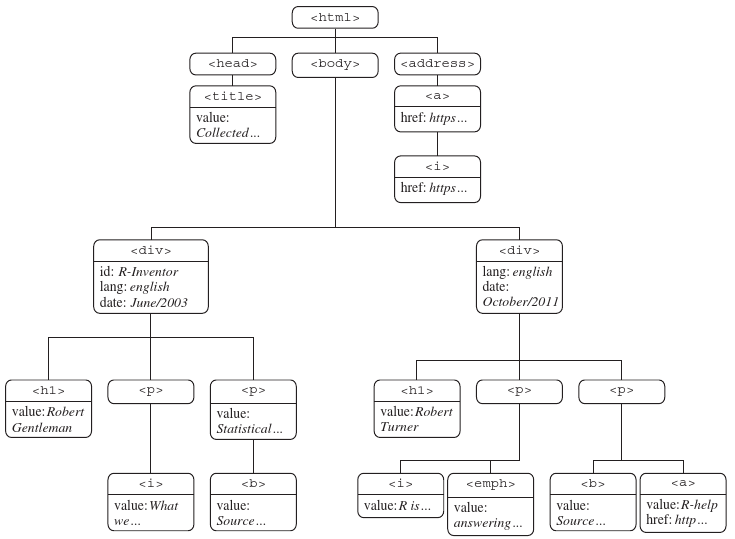
\includegraphics{tree.png}

\end{frame}

\section{Running Example}\label{running-example}

\begin{frame}[fragile]{running example}

\begin{Shaded}
\begin{Highlighting}[]
\KeywordTok{require}\NormalTok{(rvest)}
\KeywordTok{require}\NormalTok{(stringr)}
\end{Highlighting}
\end{Shaded}

\begin{Shaded}
\begin{Highlighting}[]
\NormalTok{url <-}\StringTok{ }
\StringTok{"http://pmeissner.com/downloads/fortunes.html"}
\NormalTok{fname <-}\StringTok{ }\KeywordTok{basename}\NormalTok{(url)}

\NormalTok{if(!}\KeywordTok{file.exists}\NormalTok{(fname))\{}
  \KeywordTok{download.file}\NormalTok{(url, fname)}
\NormalTok{\}}

\NormalTok{html <-}\StringTok{ }\KeywordTok{read_html}\NormalTok{(fname)}
\end{Highlighting}
\end{Shaded}

\end{frame}

\begin{frame}[fragile]{running example}

\begin{Shaded}
\begin{Highlighting}[]
\NormalTok{xml2::}\KeywordTok{html_structure}\NormalTok{(html)}
\end{Highlighting}
\end{Shaded}

\begin{verbatim}
## <html>
##   {text}
##   <head>
##     {text}
##     <title>
##       {text}
##     {text}
##     <style>
##       {cdata}
##     {text}
##   {text}
##   <body>
##     {text}
##     <div#R_Inventor [lang, date]>
##       {text}
##       <h1.pink>
##         {text}
##       {text}
##       <p>
##         {text}
##         <i>
##           {text}
##         {text}
##       {text}
##       <p>
##         {text}
##         <b.pink>
##           {text}
##         {text}
##       {text}
##     {text}
##     <div [lang, date]>
##       {text}
##       <h1.pink>
##         {text}
##       {text}
##       <p>
##         {text}
##         <i>
##           {text}
##         <br>
##         {text}
##         <emph>
##           {text}
##         {text}
##       {text}
##       <p>
##         {text}
##         <b.pink>
##           {text}
##         {text}
##         <a [href]>
##           {text}
##         {text}
##       {text}
##     {text}
##     <address>
##       {text}
##       <a [href]>
##         {text}
##         <i>
##           {text}
##         {text}
##       {text}
##     {text}
##   {text}
\end{verbatim}

\end{frame}

\section{How XPath works \ldots{}}\label{how-xpath-works}

\begin{frame}{XPath? What is it all about?}

\begin{itemize}
\tightlist
\item
  XPath is a query language for XML (Extensible Markup Language)
  documents
\item
  XML examples are:
  \href{https://en.wikipedia.org/wiki/List_of_XML_markup_languages}{XML,
  HTML, SVG, GML, KML, EPUB, RSS, Office Open XML, OpenDocument}
\item
  in XPath on selects nodes describing the paths that lead to that path
\end{itemize}

\end{frame}

\begin{frame}[fragile]{How XPath Works \ldots{}}

\begin{itemize}
\tightlist
\item
  builds on

  \begin{itemize}
  \tightlist
  \item
    \textbf{hierarchy} (select parent, child, sibling, \ldots{} node)
  \item
    \textbf{node names} (select node by name)
  \item
    \textbf{node values} (select node by value)
  \item
    \textbf{attribute name and value} (select node on attribute value)
  \item
    \textbf{further functions} (select depending on more complex
    derivates of the above)

    \begin{itemize}
    \tightlist
    \item
      e.g.~name, string\_length, contains, count, position, \ldots{}
    \end{itemize}
  \item
    \textbf{operators}

    \begin{itemize}
    \tightlist
    \item
      e.g. \texttt{\textbar{}}, \texttt{+}, \texttt{-}, \texttt{=},
      \texttt{!=}, \texttt{\textless{}=}, \texttt{or}, \texttt{and},
      \ldots{}
    \end{itemize}
  \end{itemize}
\item
  allows to extract

  \begin{itemize}
  \tightlist
  \item
    node values
  \item
    attribute values
  \end{itemize}
\item
  \ldots{} from single nodes and node sets
\end{itemize}

\end{frame}

\begin{frame}[fragile]{explicit path}

\begin{Shaded}
\begin{Highlighting}[]
\NormalTok{x=}\StringTok{"/html/body/div[2]/h1"}
\KeywordTok{html_nodes}\NormalTok{(html, }\DataTypeTok{xpath=}\NormalTok{x)}
\end{Highlighting}
\end{Shaded}

\begin{verbatim}
## {xml_nodeset (1)}
## [1] <h1 class="pink">Rolf Turner</h1>
\end{verbatim}

\end{frame}

\begin{frame}[fragile]{path anywhere in hierarchy}

\begin{Shaded}
\begin{Highlighting}[]
\KeywordTok{html_nodes}\NormalTok{(html, }\DataTypeTok{xpath=}\StringTok{"//h1"}\NormalTok{)}
\end{Highlighting}
\end{Shaded}

\begin{verbatim}
## {xml_nodeset (2)}
## [1] <h1 class="pink">Robert Gentleman</h1>
## [2] <h1 class="pink">Rolf Turner</h1>
\end{verbatim}

\end{frame}

\begin{frame}[fragile]{path anywhere in hierarchy / attribute}

\begin{Shaded}
\begin{Highlighting}[]
\KeywordTok{html_nodes}\NormalTok{(html, }\DataTypeTok{xpath=}\StringTok{"//a/@href"}\NormalTok{)}
\end{Highlighting}
\end{Shaded}

\begin{verbatim}
## {xml_nodeset (2)}
## [1]  href="https://stat.ethz.ch/mailman/listinfo/r-help"
## [2]  href="www.r-datacollectionbook.com"
\end{verbatim}

\end{frame}

\begin{frame}[fragile]{path anywhere in hierarchy / function}

\begin{Shaded}
\begin{Highlighting}[]
\KeywordTok{html_nodes}\NormalTok{(html, }\DataTypeTok{xpath=}\StringTok{"//p/i/text()"}\NormalTok{)}
\end{Highlighting}
\end{Shaded}

\begin{verbatim}
## {xml_nodeset (2)}
## [1] 'What we have is nice, but we need something very different'
## [2] 'R is wonderful, but it cannot work magic'
\end{verbatim}

\end{frame}

\begin{frame}[fragile]{path anywhere in hierarchy / indexing}

\begin{Shaded}
\begin{Highlighting}[]
\KeywordTok{html_nodes}\NormalTok{(html, }\DataTypeTok{xpath=}\StringTok{"//div[1]/p/i"}\NormalTok{)}
\end{Highlighting}
\end{Shaded}

\begin{verbatim}
## {xml_nodeset (1)}
## [1] <i>'What we have is nice, but we need something very different'</i>
\end{verbatim}

\end{frame}

\begin{frame}[fragile]{path anywhere in hierarchy / indexing}

\begin{Shaded}
\begin{Highlighting}[]
\KeywordTok{html_nodes}\NormalTok{(html, }\DataTypeTok{xpath=}\StringTok{"//div"}\NormalTok{)}
\end{Highlighting}
\end{Shaded}

\begin{verbatim}
## {xml_nodeset (2)}
## [1] <div id="R_Inventor" lang="english" date="June/2003">\n\t\t\t<h1 cla ...
## [2] <div lang="english" date="October/2011">\n\t\t\t<h1 class="pink">Rol ...
\end{verbatim}

\begin{Shaded}
\begin{Highlighting}[]
\KeywordTok{html_nodes}\NormalTok{(html, }\DataTypeTok{xpath=}\StringTok{"//div[1]"}\NormalTok{)}
\end{Highlighting}
\end{Shaded}

\begin{verbatim}
## {xml_nodeset (1)}
## [1] <div id="R_Inventor" lang="english" date="June/2003">\n\t\t\t<h1 cla ...
\end{verbatim}

\begin{Shaded}
\begin{Highlighting}[]
\KeywordTok{html_nodes}\NormalTok{(html, }\DataTypeTok{xpath=}\StringTok{"//div[1]/p/i/text()"}\NormalTok{)}
\end{Highlighting}
\end{Shaded}

\begin{verbatim}
## {xml_nodeset (1)}
## [1] 'What we have is nice, but we need something very different'
\end{verbatim}

\end{frame}

\begin{frame}[fragile]{node / attribute contains/is equal \ldots{}}

\begin{Shaded}
\begin{Highlighting}[]
\KeywordTok{html_nodes}\NormalTok{(html, }\DataTypeTok{xpath=}\StringTok{"//div[@date='October/2011']"}\NormalTok{)}
\end{Highlighting}
\end{Shaded}

\begin{verbatim}
## {xml_nodeset (1)}
## [1] <div lang="english" date="October/2011">\n\t\t\t<h1 class="pink">Rol ...
\end{verbatim}

\begin{Shaded}
\begin{Highlighting}[]
\KeywordTok{html_nodes}\NormalTok{(html, }\DataTypeTok{xpath=}\StringTok{"//div[contains(@date, 'October/2011')]"}\NormalTok{)}
\end{Highlighting}
\end{Shaded}

\begin{verbatim}
## {xml_nodeset (1)}
## [1] <div lang="english" date="October/2011">\n\t\t\t<h1 class="pink">Rol ...
\end{verbatim}

\begin{Shaded}
\begin{Highlighting}[]
\KeywordTok{html_nodes}\NormalTok{(html, }\DataTypeTok{xpath=}\StringTok{"//div[contains(.//a/@href, 'https')]"}\NormalTok{)}
\end{Highlighting}
\end{Shaded}

\begin{verbatim}
## {xml_nodeset (1)}
## [1] <div lang="english" date="October/2011">\n\t\t\t<h1 class="pink">Rol ...
\end{verbatim}

\end{frame}

\begin{frame}[fragile]{node / attribute contains/is equal \ldots{}}

\begin{Shaded}
\begin{Highlighting}[]
\KeywordTok{html_nodes}\NormalTok{(html, }\DataTypeTok{xpath=}\StringTok{"//a[contains(@href, 'https')]"}\NormalTok{)}
\end{Highlighting}
\end{Shaded}

\begin{verbatim}
## {xml_nodeset (1)}
## [1] <a href="https://stat.ethz.ch/mailman/listinfo/r-help">R-help</a>
\end{verbatim}

\begin{Shaded}
\begin{Highlighting}[]
\KeywordTok{html_nodes}\NormalTok{(html, }\DataTypeTok{xpath=}\StringTok{"//a[contains(., 'homepage')]"}\NormalTok{)}
\end{Highlighting}
\end{Shaded}

\begin{verbatim}
## {xml_nodeset (1)}
## [1] <a href="www.r-datacollectionbook.com">\n\t\t\t\t<i>The book homepag ...
\end{verbatim}

\end{frame}

\begin{frame}[fragile]{node parent}

\begin{Shaded}
\begin{Highlighting}[]
\KeywordTok{html_nodes}\NormalTok{(html, }\DataTypeTok{xpath=}\StringTok{"//a"}\NormalTok{)}
\end{Highlighting}
\end{Shaded}

\begin{verbatim}
## {xml_nodeset (2)}
## [1] <a href="https://stat.ethz.ch/mailman/listinfo/r-help">R-help</a>
## [2] <a href="www.r-datacollectionbook.com">\n\t\t\t\t<i>The book homepag ...
\end{verbatim}

\begin{Shaded}
\begin{Highlighting}[]
\KeywordTok{html_nodes}\NormalTok{(html, }\DataTypeTok{xpath=}\StringTok{"//a/.."}\NormalTok{)}
\end{Highlighting}
\end{Shaded}

\begin{verbatim}
## {xml_nodeset (2)}
## [1] <p>\n\t\t\t\t<b class="pink">Source: </b>\n\t\t\t\t<a href="https:// ...
## [2] <address>\n\t\t\t<a href="www.r-datacollectionbook.com">\n\t\t\t\t<i ...
\end{verbatim}

\end{frame}

\begin{frame}[fragile]{all nodes everywhere}

\begin{Shaded}
\begin{Highlighting}[]
\KeywordTok{html_nodes}\NormalTok{(html, }\DataTypeTok{xpath=}\StringTok{"//*"}\NormalTok{)}
\end{Highlighting}
\end{Shaded}

\begin{verbatim}
## {xml_nodeset (23)}
##  [1] <html> \n\t<head>\n\t\t<title>Collected R wisdoms</title>\n\t\t<sty ...
##  [2] <head>\n\t\t<title>Collected R wisdoms</title>\n\t\t<style><![CDATA ...
##  [3] <title>Collected R wisdoms</title>
##  [4] <style><![CDATA[\n\t\t\t.pink    {color:pink;}\n\t\t]]></style>
##  [5] <body>\n\t\t<div id="R_Inventor" lang="english" date="June/2003">\n ...
##  [6] <div id="R_Inventor" lang="english" date="June/2003">\n\t\t\t<h1 cl ...
##  [7] <h1 class="pink">Robert Gentleman</h1>
##  [8] <p>\n\t\t\t\t<i>'What we have is nice, but we need something very d ...
##  [9] <i>'What we have is nice, but we need something very different'</i>
## [10] <p>\n\t\t\t\t<b class="pink">Source: </b>Statistical Computing 2003 ...
## [11] <b class="pink">Source: </b>
## [12] <div lang="english" date="October/2011">\n\t\t\t<h1 class="pink">Ro ...
## [13] <h1 class="pink">Rolf Turner</h1>
## [14] <p>\n\t\t\t\t<i>'R is wonderful, but it cannot work magic'</i><br/> ...
## [15] <i>'R is wonderful, but it cannot work magic'</i>
## [16] <br/>
## [17] <emph>answering a request for automatic generation of 'data from a  ...
## [18] <p>\n\t\t\t\t<b class="pink">Source: </b>\n\t\t\t\t<a href="https:/ ...
## [19] <b class="pink">Source: </b>
## [20] <a href="https://stat.ethz.ch/mailman/listinfo/r-help">R-help</a>
## ...
\end{verbatim}

\end{frame}

\begin{frame}[fragile]{all nodes' text everywhere}

\begin{Shaded}
\begin{Highlighting}[]
\KeywordTok{html_nodes}\NormalTok{(html, }\DataTypeTok{xpath=}\StringTok{"//*/text()"}\NormalTok{)}
\end{Highlighting}
\end{Shaded}

\begin{verbatim}
## {xml_nodeset (43)}
##  [1]  \n\t
##  [2] \n\t\t
##  [3] Collected R wisdoms
##  [4] \n\t\t
##  [5] <![CDATA[\n\t\t\t.pink    {color:pink;}\n\t\t]]>
##  [6] \n\t
##  [7] \n\t
##  [8] \n\t\t
##  [9] \n\t\t\t
## [10] Robert Gentleman
## [11] \n\t\t\t
## [12] \n\t\t\t\t
## [13] 'What we have is nice, but we need something very different'
## [14] \n\t\t\t
## [15] \n\t\t\t
## [16] \n\t\t\t\t
## [17] Source: 
## [18] Statistical Computing 2003, Reisensburg\n\t\t\t
## [19] \n\t\t
## [20] \n\t\t
## ...
\end{verbatim}

\end{frame}

\begin{frame}[fragile]{that node or the other}

\begin{Shaded}
\begin{Highlighting}[]
\KeywordTok{html_nodes}\NormalTok{(html, }\DataTypeTok{xpath=}\StringTok{"//i | //b"}\NormalTok{)}
\end{Highlighting}
\end{Shaded}

\begin{verbatim}
## {xml_nodeset (5)}
## [1] <i>'What we have is nice, but we need something very different'</i>
## [2] <b class="pink">Source: </b>
## [3] <i>'R is wonderful, but it cannot work magic'</i>
## [4] <b class="pink">Source: </b>
## [5] <i>The book homepage</i>
\end{verbatim}

\end{frame}

\begin{frame}[fragile]{using axis :: parent}

\begin{Shaded}
\begin{Highlighting}[]
\KeywordTok{html_nodes}\NormalTok{(html, }\DataTypeTok{xpath=}\StringTok{"//a/.."}\NormalTok{)}
\end{Highlighting}
\end{Shaded}

\begin{verbatim}
## {xml_nodeset (2)}
## [1] <p>\n\t\t\t\t<b class="pink">Source: </b>\n\t\t\t\t<a href="https:// ...
## [2] <address>\n\t\t\t<a href="www.r-datacollectionbook.com">\n\t\t\t\t<i ...
\end{verbatim}

\begin{Shaded}
\begin{Highlighting}[]
\KeywordTok{html_nodes}\NormalTok{(html, }\DataTypeTok{xpath=}\StringTok{"//a/parent::*"}\NormalTok{)}
\end{Highlighting}
\end{Shaded}

\begin{verbatim}
## {xml_nodeset (2)}
## [1] <p>\n\t\t\t\t<b class="pink">Source: </b>\n\t\t\t\t<a href="https:// ...
## [2] <address>\n\t\t\t<a href="www.r-datacollectionbook.com">\n\t\t\t\t<i ...
\end{verbatim}

\begin{Shaded}
\begin{Highlighting}[]
\KeywordTok{html_nodes}\NormalTok{(html, }\DataTypeTok{xpath=}\StringTok{"//a/parent::p"}\NormalTok{)}
\end{Highlighting}
\end{Shaded}

\begin{verbatim}
## {xml_nodeset (1)}
## [1] <p>\n\t\t\t\t<b class="pink">Source: </b>\n\t\t\t\t<a href="https:// ...
\end{verbatim}

\end{frame}

\begin{frame}[fragile]{using axis :: child}

\begin{Shaded}
\begin{Highlighting}[]
\KeywordTok{html_nodes}\NormalTok{(html, }\DataTypeTok{xpath=}\StringTok{"//p/i"}\NormalTok{)}
\end{Highlighting}
\end{Shaded}

\begin{verbatim}
## {xml_nodeset (2)}
## [1] <i>'What we have is nice, but we need something very different'</i>
## [2] <i>'R is wonderful, but it cannot work magic'</i>
\end{verbatim}

\begin{Shaded}
\begin{Highlighting}[]
\KeywordTok{html_nodes}\NormalTok{(html, }\DataTypeTok{xpath=}\StringTok{"//p/child::*"}\NormalTok{)}
\end{Highlighting}
\end{Shaded}

\begin{verbatim}
## {xml_nodeset (7)}
## [1] <i>'What we have is nice, but we need something very different'</i>
## [2] <b class="pink">Source: </b>
## [3] <i>'R is wonderful, but it cannot work magic'</i>
## [4] <br/>
## [5] <emph>answering a request for automatic generation of 'data from a k ...
## [6] <b class="pink">Source: </b>
## [7] <a href="https://stat.ethz.ch/mailman/listinfo/r-help">R-help</a>
\end{verbatim}

\begin{Shaded}
\begin{Highlighting}[]
\KeywordTok{html_nodes}\NormalTok{(html, }\DataTypeTok{xpath=}\StringTok{"//p/child::i"}\NormalTok{)}
\end{Highlighting}
\end{Shaded}

\begin{verbatim}
## {xml_nodeset (2)}
## [1] <i>'What we have is nice, but we need something very different'</i>
## [2] <i>'R is wonderful, but it cannot work magic'</i>
\end{verbatim}

\end{frame}

\begin{frame}[fragile]{using axis :: ancestor}

\begin{Shaded}
\begin{Highlighting}[]
\KeywordTok{html_nodes}\NormalTok{(html, }\DataTypeTok{xpath=}\StringTok{"//b/ancestor::*"}\NormalTok{)}
\end{Highlighting}
\end{Shaded}

\begin{verbatim}
## {xml_nodeset (6)}
## [1] <html> \n\t<head>\n\t\t<title>Collected R wisdoms</title>\n\t\t<styl ...
## [2] <body>\n\t\t<div id="R_Inventor" lang="english" date="June/2003">\n\ ...
## [3] <div id="R_Inventor" lang="english" date="June/2003">\n\t\t\t<h1 cla ...
## [4] <p>\n\t\t\t\t<b class="pink">Source: </b>Statistical Computing 2003, ...
## [5] <div lang="english" date="October/2011">\n\t\t\t<h1 class="pink">Rol ...
## [6] <p>\n\t\t\t\t<b class="pink">Source: </b>\n\t\t\t\t<a href="https:// ...
\end{verbatim}

\begin{Shaded}
\begin{Highlighting}[]
\KeywordTok{html_nodes}\NormalTok{(html, }\DataTypeTok{xpath=}\StringTok{"//b/ancestor::*/text()"}\NormalTok{)}
\end{Highlighting}
\end{Shaded}

\begin{verbatim}
## {xml_nodeset (20)}
##  [1]  \n\t
##  [2] \n\t
##  [3] \n\t\t
##  [4] \n\t\t\t
##  [5] \n\t\t\t
##  [6] \n\t\t\t
##  [7] \n\t\t\t\t
##  [8] Statistical Computing 2003, Reisensburg\n\t\t\t
##  [9] \n\t\t
## [10] \n\t\t
## [11] \n\t\t\t
## [12] \n\t\t\t
## [13] \n\t\t\t
## [14] \n\t\t\t\t
## [15] \n\t\t\t\t
## [16] \n\t\t\t
## [17] \n\t\t
## [18] \n\t\t
## [19] \n\t
## [20]  \n
\end{verbatim}

\end{frame}

\begin{frame}[fragile]{using axis :: descendant}

\begin{Shaded}
\begin{Highlighting}[]
\KeywordTok{html_nodes}\NormalTok{(html, }\DataTypeTok{xpath=}\StringTok{"//p/descendant::*"}\NormalTok{)}
\end{Highlighting}
\end{Shaded}

\begin{verbatim}
## {xml_nodeset (7)}
## [1] <i>'What we have is nice, but we need something very different'</i>
## [2] <b class="pink">Source: </b>
## [3] <i>'R is wonderful, but it cannot work magic'</i>
## [4] <br/>
## [5] <emph>answering a request for automatic generation of 'data from a k ...
## [6] <b class="pink">Source: </b>
## [7] <a href="https://stat.ethz.ch/mailman/listinfo/r-help">R-help</a>
\end{verbatim}

\begin{Shaded}
\begin{Highlighting}[]
\KeywordTok{html_nodes}\NormalTok{(html, }\DataTypeTok{xpath=}\StringTok{"//p/descendant::*/text()"}\NormalTok{)}
\end{Highlighting}
\end{Shaded}

\begin{verbatim}
## {xml_nodeset (6)}
## [1] 'What we have is nice, but we need something very different'
## [2] Source: 
## [3] 'R is wonderful, but it cannot work magic'
## [4] answering a request for automatic generation of 'data from a known m ...
## [5] Source: 
## [6] R-help
\end{verbatim}

\end{frame}

\begin{frame}[fragile]{using axis :: following-sibling /
preceding-sibling}

\begin{Shaded}
\begin{Highlighting}[]
\KeywordTok{html_nodes}\NormalTok{(html, }\DataTypeTok{xpath=}\StringTok{"//b/.."}\NormalTok{)}
\end{Highlighting}
\end{Shaded}

\begin{verbatim}
## {xml_nodeset (2)}
## [1] <p>\n\t\t\t\t<b class="pink">Source: </b>Statistical Computing 2003, ...
## [2] <p>\n\t\t\t\t<b class="pink">Source: </b>\n\t\t\t\t<a href="https:// ...
\end{verbatim}

\begin{Shaded}
\begin{Highlighting}[]
\KeywordTok{html_nodes}\NormalTok{(html, }\DataTypeTok{xpath=}\StringTok{"//b/following-sibling::*"}\NormalTok{)}
\end{Highlighting}
\end{Shaded}

\begin{verbatim}
## {xml_nodeset (1)}
## [1] <a href="https://stat.ethz.ch/mailman/listinfo/r-help">R-help</a>
\end{verbatim}

\end{frame}

\section{How CSS-Selectors Work \ldots{}}\label{how-css-selectors-work}

\begin{frame}{How CSS-Selectors Work \ldots{}}

\begin{itemize}
\tightlist
\item
  CSS-Selectors were designed to apply Styles to HTML elements
\item
  While XPath is build around the idea of hierarchy and tree-structure
  first and foremost meaning that paths lead to data, with CSS-S
  selection is more set-like.
\item
  CSS-S is used and written for Web-Designers so it might be
  less-powerful-complete-systematic than XPath but it is also less
  intimidating and easier to write
\item
  selection on class and id attributes is super easy

  \begin{itemize}
  \tightlist
  \item
    \textbf{name} (select nodes by name)
  \item
    \textbf{id} (select node id attribute)
  \item
    \textbf{node values} (select node by value)
  \item
    \textbf{attribute name and value} (select node on attribute value)
  \item
    \textbf{hierarchy} (select depending on the position in path)
  \end{itemize}
\end{itemize}

\end{frame}

\begin{frame}[fragile]{selecting nodes by name}

\begin{Shaded}
\begin{Highlighting}[]
\KeywordTok{html_nodes}\NormalTok{(html, }\StringTok{"p"}\NormalTok{)}
\end{Highlighting}
\end{Shaded}

\begin{verbatim}
## {xml_nodeset (4)}
## [1] <p>\n\t\t\t\t<i>'What we have is nice, but we need something very di ...
## [2] <p>\n\t\t\t\t<b class="pink">Source: </b>Statistical Computing 2003, ...
## [3] <p>\n\t\t\t\t<i>'R is wonderful, but it cannot work magic'</i><br/>\ ...
## [4] <p>\n\t\t\t\t<b class="pink">Source: </b>\n\t\t\t\t<a href="https:// ...
\end{verbatim}

\begin{Shaded}
\begin{Highlighting}[]
\KeywordTok{html_nodes}\NormalTok{(html, }\StringTok{"b, i"}\NormalTok{)}
\end{Highlighting}
\end{Shaded}

\begin{verbatim}
## {xml_nodeset (5)}
## [1] <i>'What we have is nice, but we need something very different'</i>
## [2] <b class="pink">Source: </b>
## [3] <i>'R is wonderful, but it cannot work magic'</i>
## [4] <b class="pink">Source: </b>
## [5] <i>The book homepage</i>
\end{verbatim}

\end{frame}

\begin{frame}[fragile]{selecting nodes by class}

\begin{Shaded}
\begin{Highlighting}[]
\KeywordTok{html_nodes}\NormalTok{(html, }\StringTok{".pink"}\NormalTok{)}
\end{Highlighting}
\end{Shaded}

\begin{verbatim}
## {xml_nodeset (4)}
## [1] <h1 class="pink">Robert Gentleman</h1>
## [2] <b class="pink">Source: </b>
## [3] <h1 class="pink">Rolf Turner</h1>
## [4] <b class="pink">Source: </b>
\end{verbatim}

\end{frame}

\begin{frame}[fragile]{selecting nodes by id}

\begin{Shaded}
\begin{Highlighting}[]
\KeywordTok{html_nodes}\NormalTok{(html, }\DataTypeTok{css =} \StringTok{"#R_Inventor"}\NormalTok{)}
\end{Highlighting}
\end{Shaded}

\begin{verbatim}
## {xml_nodeset (1)}
## [1] <div id="R_Inventor" lang="english" date="June/2003">\n\t\t\t<h1 cla ...
\end{verbatim}

\begin{Shaded}
\begin{Highlighting}[]
\KeywordTok{html_nodes}\NormalTok{(html, }\DataTypeTok{css =} \StringTok{"[id='R_Inventor']"}\NormalTok{)}
\end{Highlighting}
\end{Shaded}

\begin{verbatim}
## {xml_nodeset (1)}
## [1] <div id="R_Inventor" lang="english" date="June/2003">\n\t\t\t<h1 cla ...
\end{verbatim}

\end{frame}

\begin{frame}[fragile]{selecting nodes by attribute}

\begin{Shaded}
\begin{Highlighting}[]
\KeywordTok{html_nodes}\NormalTok{(html, }\DataTypeTok{css =} \StringTok{"[lang]"}\NormalTok{)}
\end{Highlighting}
\end{Shaded}

\begin{verbatim}
## {xml_nodeset (2)}
## [1] <div id="R_Inventor" lang="english" date="June/2003">\n\t\t\t<h1 cla ...
## [2] <div lang="english" date="October/2011">\n\t\t\t<h1 class="pink">Rol ...
\end{verbatim}

\begin{Shaded}
\begin{Highlighting}[]
\KeywordTok{html_nodes}\NormalTok{(html, }\DataTypeTok{css =} \StringTok{"[href]"}\NormalTok{)}
\end{Highlighting}
\end{Shaded}

\begin{verbatim}
## {xml_nodeset (2)}
## [1] <a href="https://stat.ethz.ch/mailman/listinfo/r-help">R-help</a>
## [2] <a href="www.r-datacollectionbook.com">\n\t\t\t\t<i>The book homepag ...
\end{verbatim}

\end{frame}

\begin{frame}[fragile]{selecting nodes by attribute value}

\begin{Shaded}
\begin{Highlighting}[]
\KeywordTok{html_nodes}\NormalTok{(html, }\DataTypeTok{css =} \StringTok{"[id=R_Inventor]"}\NormalTok{) }\CommentTok{# equal}
\end{Highlighting}
\end{Shaded}

\begin{verbatim}
## {xml_nodeset (1)}
## [1] <div id="R_Inventor" lang="english" date="June/2003">\n\t\t\t<h1 cla ...
\end{verbatim}

\begin{Shaded}
\begin{Highlighting}[]
\KeywordTok{html_nodes}\NormalTok{(html, }\DataTypeTok{css =} \StringTok{"[id^=R]"}\NormalTok{)         }\CommentTok{# starts }
\end{Highlighting}
\end{Shaded}

\begin{verbatim}
## {xml_nodeset (1)}
## [1] <div id="R_Inventor" lang="english" date="June/2003">\n\t\t\t<h1 cla ...
\end{verbatim}

\begin{Shaded}
\begin{Highlighting}[]
\KeywordTok{html_nodes}\NormalTok{(html, }\DataTypeTok{css =} \StringTok{"[id$=r]"}\NormalTok{)         }\CommentTok{# ends}
\end{Highlighting}
\end{Shaded}

\begin{verbatim}
## {xml_nodeset (1)}
## [1] <div id="R_Inventor" lang="english" date="June/2003">\n\t\t\t<h1 cla ...
\end{verbatim}

\begin{Shaded}
\begin{Highlighting}[]
\KeywordTok{html_nodes}\NormalTok{(html, }\DataTypeTok{css =} \StringTok{"[id*=ven]"}\NormalTok{)       }\CommentTok{# conatains}
\end{Highlighting}
\end{Shaded}

\begin{verbatim}
## {xml_nodeset (1)}
## [1] <div id="R_Inventor" lang="english" date="June/2003">\n\t\t\t<h1 cla ...
\end{verbatim}

\end{frame}

\begin{frame}[fragile]{selecting nodes by path characteristics :
decendant}

\begin{Shaded}
\begin{Highlighting}[]
\KeywordTok{html_nodes}\NormalTok{(html, }\DataTypeTok{css =} \StringTok{"i"}\NormalTok{)}
\end{Highlighting}
\end{Shaded}

\begin{verbatim}
## {xml_nodeset (3)}
## [1] <i>'What we have is nice, but we need something very different'</i>
## [2] <i>'R is wonderful, but it cannot work magic'</i>
## [3] <i>The book homepage</i>
\end{verbatim}

\begin{Shaded}
\begin{Highlighting}[]
\KeywordTok{html_nodes}\NormalTok{(html, }\DataTypeTok{css =} \StringTok{"a i"}\NormalTok{)}
\end{Highlighting}
\end{Shaded}

\begin{verbatim}
## {xml_nodeset (1)}
## [1] <i>The book homepage</i>
\end{verbatim}

\end{frame}

\begin{frame}[fragile]{selecting nodes by path characteristics :parent}

\begin{Shaded}
\begin{Highlighting}[]
\KeywordTok{html_nodes}\NormalTok{(html, }\DataTypeTok{css =} \StringTok{"p > i"}\NormalTok{)}
\end{Highlighting}
\end{Shaded}

\begin{verbatim}
## {xml_nodeset (2)}
## [1] <i>'What we have is nice, but we need something very different'</i>
## [2] <i>'R is wonderful, but it cannot work magic'</i>
\end{verbatim}

\begin{Shaded}
\begin{Highlighting}[]
\KeywordTok{html_nodes}\NormalTok{(html, }\DataTypeTok{css =} \StringTok{"a > i"}\NormalTok{)}
\end{Highlighting}
\end{Shaded}

\begin{verbatim}
## {xml_nodeset (1)}
## [1] <i>The book homepage</i>
\end{verbatim}

\end{frame}

\begin{frame}[fragile]{selecting nodes by path characteristics : first
of type}

\begin{Shaded}
\begin{Highlighting}[]
\KeywordTok{html_nodes}\NormalTok{(html, }\DataTypeTok{css =} \StringTok{"p:first-of-type"}\NormalTok{)}
\end{Highlighting}
\end{Shaded}

\begin{verbatim}
## {xml_nodeset (2)}
## [1] <p>\n\t\t\t\t<i>'What we have is nice, but we need something very di ...
## [2] <p>\n\t\t\t\t<i>'R is wonderful, but it cannot work magic'</i><br/>\ ...
\end{verbatim}

\end{frame}

\begin{frame}[fragile]{selecting nodes by path characteristics : nth
child of parent}

\begin{Shaded}
\begin{Highlighting}[]
\KeywordTok{html_nodes}\NormalTok{(html, }\DataTypeTok{css =} \StringTok{"a:nth-child(1)"}\NormalTok{)}
\end{Highlighting}
\end{Shaded}

\begin{verbatim}
## {xml_nodeset (1)}
## [1] <a href="www.r-datacollectionbook.com">\n\t\t\t\t<i>The book homepag ...
\end{verbatim}

\begin{Shaded}
\begin{Highlighting}[]
\KeywordTok{html_nodes}\NormalTok{(html, }\DataTypeTok{css =} \StringTok{"a:nth-child(2)"}\NormalTok{)}
\end{Highlighting}
\end{Shaded}

\begin{verbatim}
## {xml_nodeset (1)}
## [1] <a href="https://stat.ethz.ch/mailman/listinfo/r-help">R-help</a>
\end{verbatim}

\end{frame}

\begin{frame}[fragile]{selecting nodes by path characteristics : nth
child of parent}

\begin{Shaded}
\begin{Highlighting}[]
\KeywordTok{html_nodes}\NormalTok{(html, }\DataTypeTok{css =} \StringTok{"a:nth-last-child(1)"}\NormalTok{)}
\end{Highlighting}
\end{Shaded}

\begin{verbatim}
## {xml_nodeset (2)}
## [1] <a href="https://stat.ethz.ch/mailman/listinfo/r-help">R-help</a>
## [2] <a href="www.r-datacollectionbook.com">\n\t\t\t\t<i>The book homepag ...
\end{verbatim}

\begin{Shaded}
\begin{Highlighting}[]
\KeywordTok{html_nodes}\NormalTok{(html, }\DataTypeTok{css =} \StringTok{"a:nth-last-child(2)"}\NormalTok{)}
\end{Highlighting}
\end{Shaded}

\begin{verbatim}
## {xml_nodeset (0)}
\end{verbatim}

\end{frame}

\begin{frame}[fragile]{selecting nodes by path characteristics : nth
child of parent}

\begin{Shaded}
\begin{Highlighting}[]
\KeywordTok{html_nodes}\NormalTok{(html, }\DataTypeTok{css =} \StringTok{"p:nth-of-type(1)"}\NormalTok{)}
\end{Highlighting}
\end{Shaded}

\begin{verbatim}
## {xml_nodeset (2)}
## [1] <p>\n\t\t\t\t<i>'What we have is nice, but we need something very di ...
## [2] <p>\n\t\t\t\t<i>'R is wonderful, but it cannot work magic'</i><br/>\ ...
\end{verbatim}

\end{frame}

\section{R-Packages and Functions}\label{r-packages-and-functions}

\begin{frame}{rvest and XML}

\textbf{rvest} (httr + xml2 + selectr)

\begin{itemize}
\tightlist
\item
  scraping centered package (download and extraction)
\item
  HTML / XML
\item
  XPath / CSS-S
\item
  very handy and slick
\item
  we use this
\end{itemize}

\textbf{XML} (xml)

\begin{itemize}
\tightlist
\item
  XML centered package (parsing and extraction)
\item
  XPath
\item
  much more powerful in terms of parsing (also SAX for LARGE documents)
\item
  goes back to 1999 (according to README; you know just after the
  internet became a thing)
\item
  two good sources cover that one: Nolan \& Temple-Lang (2013):
  \emph{XML and Web Technologies for Data Sciences with R}; Munzert et
  al (2014): \emph{Automated Data Collection with R}
\end{itemize}

\end{frame}

\begin{frame}[fragile]{rvest's (important) XML handling functions}

\begin{longtable}[c]{@{}ll@{}}
\toprule
function & description\tabularnewline
\midrule
\endhead
\texttt{read\_html()} & parse HTML (file); all others based
on\tabularnewline
\texttt{html\_structure()} & shows the structure of an HTML
(doc)\tabularnewline
\texttt{as\_list()} & transform parsed XML / HTML to list
(doc)\tabularnewline
\texttt{html\_attr()} & get specific attribute value
(node)\tabularnewline
\texttt{html\_attrs()} & get all attributes (node)\tabularnewline
\texttt{html\_text()} & get node's and children's text
(node)\tabularnewline
\texttt{html\_children()} & get children of node (doc,
node)\tabularnewline
\texttt{xml\_path()} & gives back the explicit path to nodes
(node)\tabularnewline
\texttt{xml\_length()} & number of children (node)\tabularnewline
\texttt{html\_name()} & name of nodes (node)\tabularnewline
\texttt{xml\_parent()} & gives back parent of node (node)\tabularnewline
\texttt{xml\_parents()} & gives back all ancestors of node
(node)\tabularnewline
\texttt{xml\_siblings()} & gives back nodes with the same parent
(node)\tabularnewline
\texttt{xml\_type()} & gives back type (node, doc)\tabularnewline
\bottomrule
\end{longtable}

doc: parsed document; node: node set or node; file: un-parsed XML
document

\end{frame}

\section{Selector Gadget and Developer Tools to the
Rescue}\label{selector-gadget-and-developer-tools-to-the-rescue}

\begin{frame}{Selector Gadget and Developer Tools to the Rescue}

\begin{itemize}
\tightlist
\item
  building Xpath (CSS-S) expressions is an art (practice hard and be
  creative)
\item
  \ldots{} and easily and quickly becomes mind buggling and complicated
  \ldots{}
\item
  \ldots{} there are however some tools that might help lessen the
  burden:

  \begin{itemize}
  \tightlist
  \item
    selectorgadget : \url{http://selectorgadget.com/}
  \item
    developer tools :

    \begin{itemize}
    \tightlist
    \item
      Firefox: \url{https://developer.mozilla.org/de/docs/Tools}
    \item
      Chrome: \url{https://developer.chrome.com/devtools}
    \item
      Safari: \url{https://developer.apple.com/safari/tools/}
    \item
      Opera: \url{http://www.opera.com/dragonfly/}
    \item
      Edge:
      \url{https://dev.windows.com/en-us/microsoft-edge/platform/documentation/f12-devtools-guide/}
    \end{itemize}
  \end{itemize}
\end{itemize}

\end{frame}

\end{document}
